\newpage




\section{Pointer Analysis}

Pointer analysis is a compile-time technique that helps identify relationships between pointer variables and the memory locations that
they point to during program execution. Pointers are powerful programming constructs and allow complex memory manipulation during program
execution through techniques such as pointer arithmetic and dynamic memory allocation. Pointer relationships can thus be complex and difficult
to analyze at compile time. On the other hand, however, they provide the benefit of simplifying various other compile time analyses such as
constant propagation, alias analysis in C programs that allow extensive use of pointers.\cite{Pointsto7:online}



Potential applications of pointer analysis for multithreaded programs include:
the development of sophisticated software engineering tools such as race detectors, memory leak detectors, wild pointer detectors and program slicers;
memory system optimizations such as prefetching
and moving computation to remote data; automatic batching of long latency
file system operations; support parallelism in different levels: instruction-level parallelism and thread-level parallelism ;
and to provide information required to apply traditional
compiler optimizations such as constant propagation, common subexpression
elimination, register allocation, code motion and induction variable elimination
to multithreaded programs.\cite{rugina2003pointer}

\begin{definition}{Aliases}
	Two variables are aliases if they reference the same memory location.
\end{definition}


\begin{definition}{The	Pointer	Alias	Analysis	Problem	}
	Decide for every pair of pointers at every program point: do they point to the same memory location?
\end{definition}

\subsection{Background}

A pointer alias analysis attempts to determine when two pointer expressions refer to the same storage location. A
points-to analysis , or similarly, an analysis based
on a compact representation , attempts to determine what storage locations a pointer can point to. This
information can then be used to determine the aliases in the program. Alias information is central to determining what
memory locations are modifed or referenced.

There are several dimensions that aect the cost/precision
trade-offs of interprocedural pointer analyses. How a pointer
analysis addresses each of these dimensions helps to categorized the analysis. An empirical comparison with a
difference in more than one dimension can limit the usefulness of
the comparison. Some of the dimensions are

\textbf{ Flow-sensitivity:} Is control-ow information of a procedure used during the analysis? By not considering control
ow information, and therefore computing a conservative
summary, ow-insensitive analyses compute one solution for
either the whole program or for each method, whereas a ow-sensitive analysis computes a solution for each program point.
Flow-insensitive analyses thus can be more efficient, but less precise than a ow-sensitive analysis. Flow-insensitive analyses
are either equality-based, which treat assignments as bidirectional and typically use a union-find data structure,
or subset-based, which treat an assignment as
a unidirectional ow of values.

\textbf{ Context-sensitivity:} Is calling context considered when
analyzing a function or can values ow from one call through
the function and return to another caller?

\textbf{ Heap modeling:} Are ob jects named by allocation site,
or is a more sophisticated shape analysis performed?

\textbf{ Aggregate modeling:} Are elements of aggregates distinguished or collapsed into one object?

\textbf{ Whole program:} Does an analysis require the whole
program or can a sound solution be obtained by analyzing
only components of a program?

\textbf{ Alias representation:} Is an explicit alias representation [51, 64] or a points-to/compact representation used?


\subsection{Flow-Sensitivity}

Flow-sensitive pointer analysis respects a program’s control flow
and computes a separate solution for each program point, in contrast to a flow-insensitive analysis,
which ignores statement ordering and computes a single solution that is conservatively correct for
all program points.


\begin{figure}[H]
	\centering
	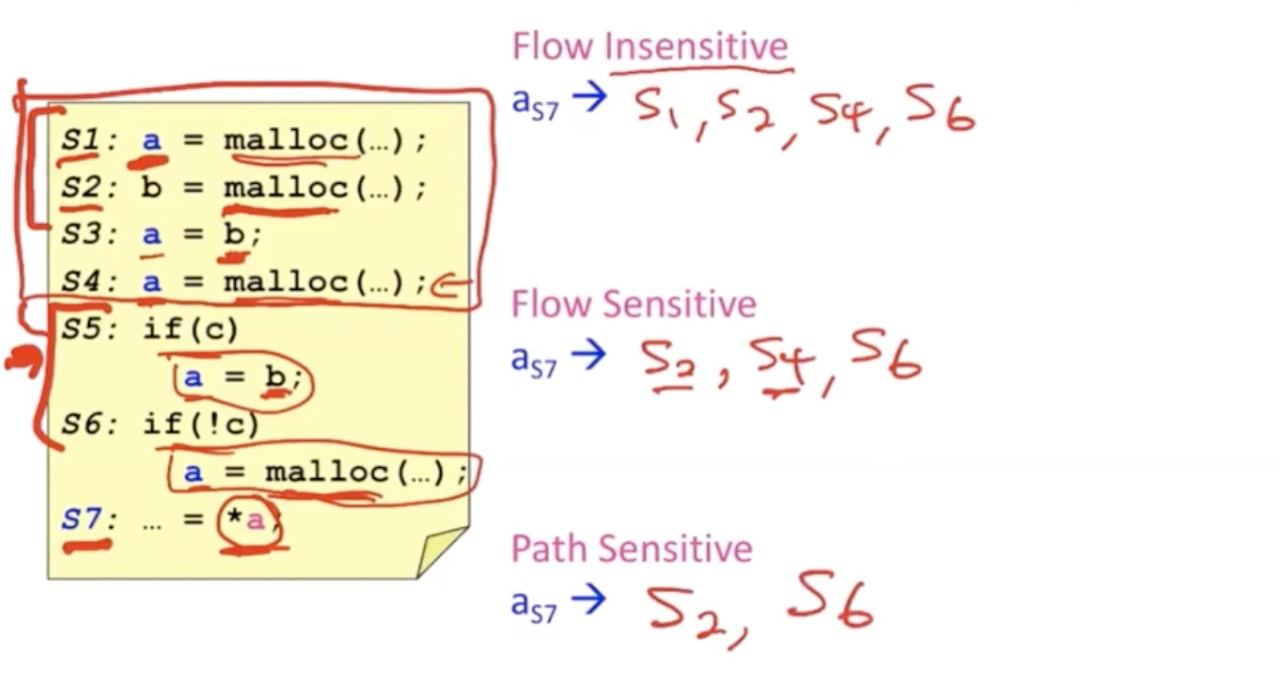
\includegraphics[width=0.7\textwidth]{p127.jpg}
	\caption{Flow-sensitive vs. flow-insensitive analysis}
	\label{fig:p127}
\end{figure}


\subsection{Context-sensitive }


Context sensitivity has a most significant impact on analysis precision due to separate
treatment for each method in the program. In practice, each time analysis considers new
method call it creates a new structure that represents unique method scope in the memory.
It treats all read/write operations inside this method in scope of this context and makes this
information available later for its processing.


\begin{figure}[H]
	\centering
	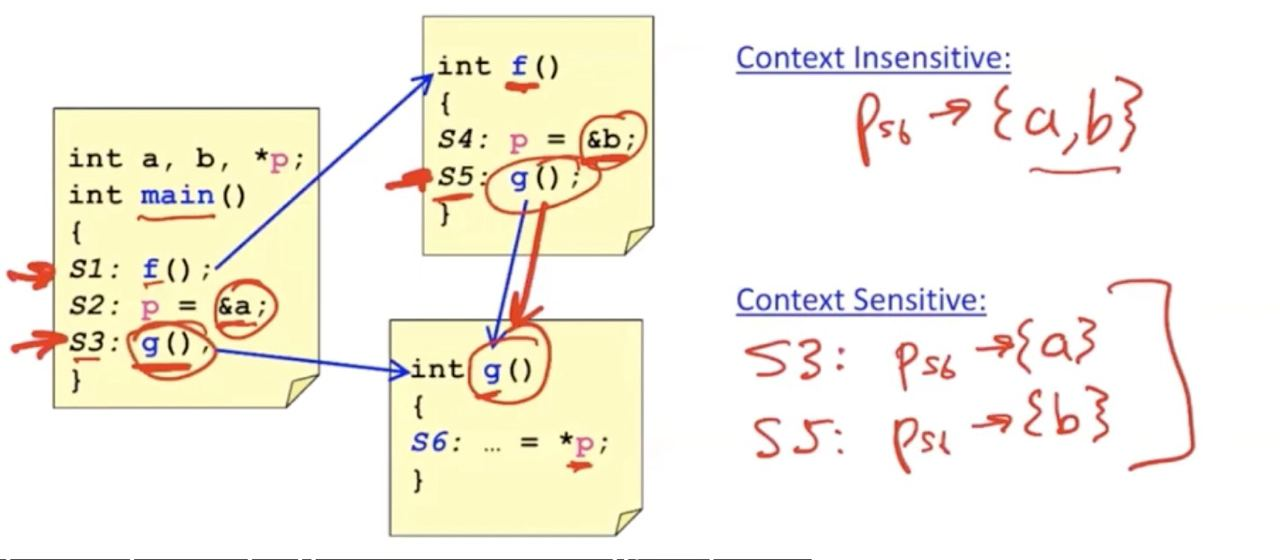
\includegraphics[width=0.7\textwidth]{p128.jpg}
	\caption{Context-sensitive vs. Context-insensitive analysis}
	\label{fig:p128}
\end{figure}



\subsection{Modeling Aggregates}
A key implementation detail is whether aggregate com-
ponents are distinguished or summarized into one object.
C/C++'s weak typing makes this diÆcult to address cor-
rectly. Thus, most published work does not distinguish ag-
gregates. However, this diÆculty does not exist in a strongly-
type language like Java, and therefore, components should
be distinguished in such languages. Most recent work
has chosen to distinguish components. Unfortunately, few researchers have studied the impact of this decision.



\subsection{Andersen’s Points-To Analysis}

\cite{notes07p17:online}Two common kinds of pointer analysis are alias analysis and points-to analysis. Alias analysis
computes sets S holding pairs of variables pp, qq, where p and q may (or must) point to the same
location. Points-to analysis, as described above, computes a relation points-topp, xq, where p may
(or must) point to the location of the variable x. We will focus primarily on points-to analysis,
beginning with a simple but useful approach originally proposed by Andersen (PhD thesis:
“Program Analysis and Specialization for the C Programming Language”).
Our initial setting will be C programs. We are interested in analyzing instructions that are
relevant to pointers in the program. Ignoring for the moment memory allocation and arrays, we
can decompose all pointer operations into four types: taking the address of a variable, copying a
pointer from one variable to another, assigning through a pointer, and dereferencing a pointer:


\begin{figure}[H]
	\centering
	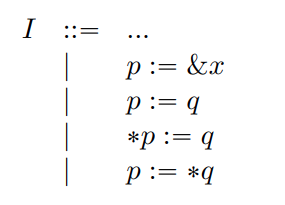
\includegraphics[width=0.25\textwidth]{p129.png}
	\label{fig:p129}
\end{figure}


Andersen’s points-to analysis is a context-insensitive interprocedural analysis. It is also a flowinsensitive analysis, that is an analysis that does not consider program statement order. Contextand flow-insensitivity are used to improve the performance of the analysis, as precise pointer
analysis can be notoriously expensive in practice.

We will formulate Andersen’s analysis by generating set constraints which can later be processed by a set constraint solver using a number of technologies. Constraint generation for each
statement works as given in the following set of rules. Because the analysis is flow-insensitive,
we do not care what order the instructions in the program come in; we simply generate a set of
constraints and solve them.


\begin{figure}[H]
	\centering
	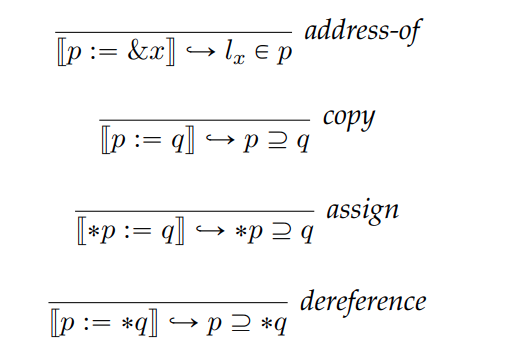
\includegraphics[width=0.4\textwidth]{p130.png}
	\label{fig:p130}
\end{figure}
% $$
% \begin{gathered}
% \overline{\llbracket p:=\& x \rrbracket \hookrightarrow l_x \in p} \text { address-of } \\
% \overline{\llbracket p:=q \rrbracket \hookrightarrow p \supseteq q} \text { copy } \\
% \overline{\llbracket * p:=q \rrbracket \hookrightarrow * p \supseteq q} \text { assign } \\
% \overline{\llbracket p:=* q \rrbracket \hookrightarrow p \supseteq * q} \text { dereference }
% \end{gathered}
% $$

The constraints generated are all set constraints. The first rule states that a constant location lx,
representation the address of x, is in the set of location pointed to by p. The second rule states that
the set of locations pointed to by p must be a superset of those pointed to by q. The last two rules
state the same, but take into account that one or the other pointer is dereferenced.

A number of specialized set constraint solvers exist and constraints in the form above can be
translated into the input for these. The dereference operation (the * in *p $\subseteq$ q)
is not standard in set constraints, but it can be encoded—see Fahndrich’s Ph.D. thesis for an example of how ¨
to encode Andersen’s points-to analysis for the BANE constraint solving engine. We will treat
constraint-solving abstractly using the following constraint propagation rules:


\begin{figure}[H]
	\centering
	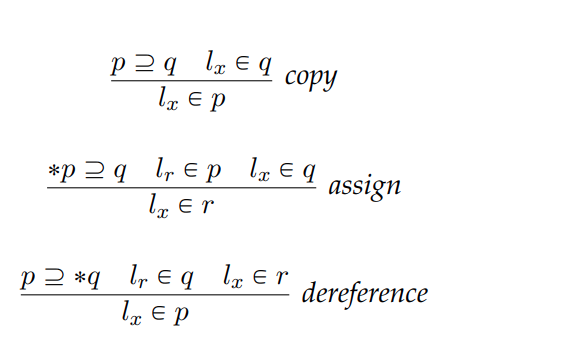
\includegraphics[width=0.4\textwidth]{p131.png}
	\caption{}
	\label{fig:p131}
\end{figure}

We can also apply Andersen’s analysis to programs with dynamic memory allocation, such as:



\begin{figure}[H]
	\centering
	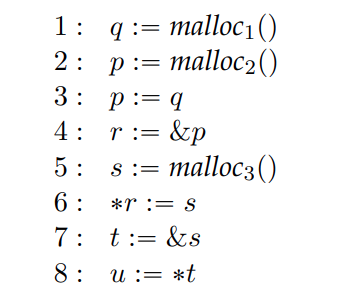
\includegraphics[width=0.3\textwidth]{p132.png}
	\caption{}
	\label{fig:p132}
\end{figure}


In this example, the analysis is run the same way, but we treat the memory cell allocated at
each malloc or new statement as an abstract location labeled by the location n of the allocation
point. We can use the rules:


\begin{figure}[H]
	\centering
	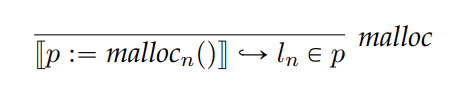
\includegraphics[width=0.4\textwidth]{p133.png}
	\caption{}
	\label{fig:p133}
\end{figure}



We must be careful because a malloc statement can be executed more than once, and each time
it executes, a new memory cell is allocated. Unless we have some other means of proving that
the malloc executes only once, we must assume that if some variable p only points to one abstract
malloc’d location $l_n$, that is still may-alias information (i.e. p points to only one of the many actual
cells allocated at the given program location) and not must-alias information.


Analyzing the efficiency of Andersen’s algorithm, we can see that all
constraints can be generated in a linear $O(n)$ pass over the program.
The solution size is $O(n^2)$ because each of the $O(n)$
variables defined in the program could potentially point to $O(n)$ other variables.


We can derive the execution time from a theorem by David McAllester published in SAS’99.
There are $O(n)$ flow constraints generated of the form
p $\subseteq$ q, *p $\subseteq$ q, or p $\subseteq$ *q. How many
times could a constraint propagation rule fire for each flow constraint?
For a p $\subseteq$ q constraint,
the rule may fire at most $O(n)$ times, because there are at most $O(n)$ premises of the proper form
$l_x \in p$. However, a constraint of the form p $\subseteq$ *q could cause
$O(n^2)$ rule firings, because there
are $O(n)$ premises each of the form $l_x \in p$ and$l_r \in q$.
With $O(n)$ constraints of the form p $\subseteq$ *q
and $O(n^2)$firings for each, we have $O(n^3)$ constraint firings overall.
A similar analysis applies for
*p $\subseteq$ q constraints. McAllester’s theorem states that the analysis with $O(n^3)$ rule firings can be
implemented in $O(n^3)$ time. Thus we have derived that Andersen’s algorithm is cubic in the size
of the program, in the worst case.



\subsubsection{Field-Sensitive Analysis}

What happens when we have a pointer to a struct in C, or an object in an object-oriented language?
In this case, we would like the pointer analysis to tell us what each field in the struct or object
points to. A simple solution is to be field-insensitive, treating all fields in a struct as equivalent.
Thus if p points to a struct with two fields f and g, and we assign:

\begin{figure}[H]
	\centering
	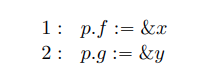
\includegraphics[width=0.4\textwidth]{p134.png}
	\caption{}
	\label{fig:p134}
\end{figure}


A field-insensitive analysis would tell us (imprecisely) that p.f could point to y. In order
to be more precise, we can track the contents each field of each abstract location separately. In
the discussion below, we assume a setting in which we cannot take the address of a field; this
assumption is true for Java but not for C. We can define a new kind of constraints for fields:


\begin{figure}[H]
	\centering
	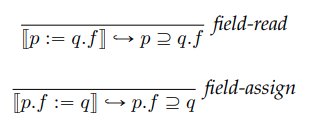
\includegraphics[width=0.4\textwidth]{p135.png}
	\caption{}
	\label{fig:p135}
\end{figure}

Now assume that objects (e.g. in Java) are represented by abstract locations l. We can process
field constraints with the following rules:

\begin{figure}[H]
	\centering
	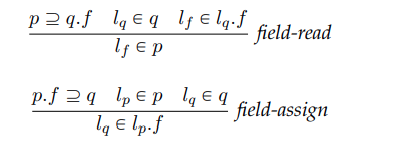
\includegraphics[width=0.4\textwidth]{p136.png}
	\caption{}
	\label{fig:p136}
\end{figure}


If we run this analysis on the code above, we find that it can distinguish that p.f points to x
and p.g points to y.


\subsection{Steensgaard’s Points-To Analysis}

For large programs, a cubic algorithm is too inefficient. Steensgaard proposed an pointer analysis
algorithm that operates in near-linear time, supporting essentially unlimited scalability in practice.
The first challenge in designing a near-linear time points-to analysis is to represent the results
in linear space. This is nontrivial because over the course of program execution, any given pointer
p could potentially point to the location of any other variable or pointer q. Representing all of
these pointers explicitly will inherently take $O(n^2)$space.
The solution Steensgaard found is based on using constant space for each variable in the program. His analysis associates each variable p with an abstract location named after the variable.
Then, it tracks a single points-to relation between that abstract location p and another one q, to
which it may point. Now, it is possible that in some real program p may point to both q and some
other variable r. In this situation, Steensgaard’s algorithm unifies the abstract locations for q and
r, creating a single abstract location representing both of them. Now we can track the fact that p
may point to either variable using a single points-to relationship.

For example, consider the program below:

\begin{figure}[H]
	\centering
	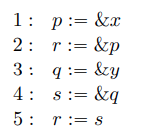
\includegraphics[width=0.3\textwidth]{p137.png}
	\caption{}
	\label{fig:p137}
\end{figure}

Andersen’s points-to analysis would produce the following graph:
\begin{figure}[H]
	\centering
	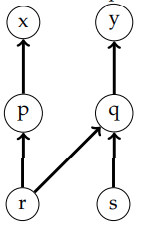
\includegraphics[width=0.3\textwidth]{p138.png}
	\caption{}
	\label{fig:p138}
\end{figure}

But in Steensgaard’s setting, when we discover that r could point both to q and to p, we must
merge q and p into a single node:

\begin{figure}[H]
	\centering
	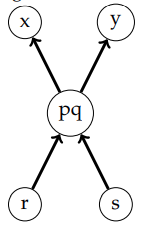
\includegraphics[width=0.3\textwidth]{p139.png}
	\caption{}
	\label{fig:p139}
\end{figure}


Notice that we have lost precision: by merging the nodes for p and q our graph now implies
that s could point to p, which is not the case in the actual program. But we are not done. Now
pq has two outgoing arrows, so we must merge nodes x and y. The final graph produced by
Steensgaard’s algorithm is therefore:

\begin{figure}[H]
	\centering
	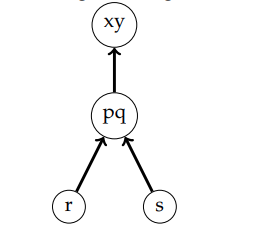
\includegraphics[width=0.3\textwidth]{p140.png}
	\caption{}
	\label{fig:p140}
\end{figure}

To define Steensgaard’s analysis more precisely, we will study a simplified version of that
ignores function pointers. It can be specified as follows:

\begin{figure}[H]
	\centering
	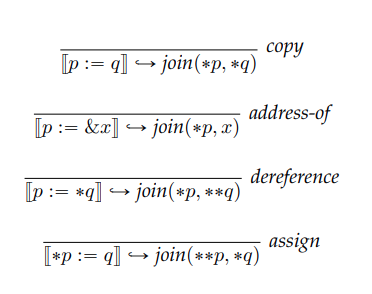
\includegraphics[width=0.3\textwidth]{p141.png}
	\caption{}
	\label{fig:p141}
\end{figure}

With each abstract location p, we associate the abstract location that p 
points to, denoted *p.
Abstract locations are implemented as a union-find data structure so that we can merge two
abstract locations efficiently. In the rules above, we implicitly invoke find on an abstract location
before calling join on it, or before looking up the location it points to.

The join operation essentially implements a union operation on the abstract locations. However, since we are tracking what each abstract location points to, we must update this information
also. The algorithm to do so is as follows:

\begin{figure}[H]
	\centering
	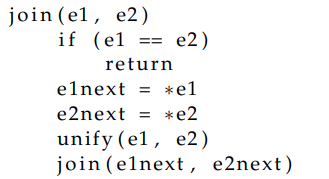
\includegraphics[width=0.3\textwidth]{p142.png}
	\caption{}
	\label{fig:p142}
\end{figure}


Once again, we implicitly invoke find on an abstract location before comparing it for equality,
looking up the abstract location it points to, or calling join recursively.


As an optimization, Steensgaard does not perform the join if the right hand side is not a pointer.
For example, if we have an assignment p := q and q has not been assigned any pointer value so
far in the analysis, we ignore the assignment. If later we find that q may hold a pointer, we must
revisit the assignment to get a sound result.

Steensgaard illustrated his algorithm using the following program:


\begin{figure}[H]
	\centering
	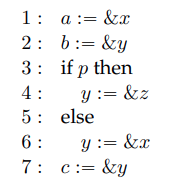
\includegraphics[width=0.3\textwidth]{p143.png}
	\caption{}
	\label{fig:p143}
\end{figure}

His analysis produces the following graph for this program:

\begin{figure}[H]
	\centering
	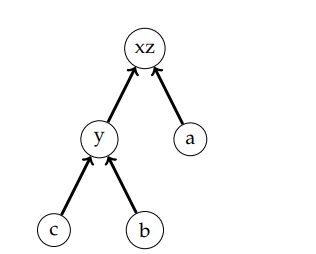
\includegraphics[width=0.3\textwidth]{p144.png}
	\caption{}
	\label{fig:p144}
\end{figure}

Rayside illustrates a situation in which Andersen must do more work than Steensgaard:


\begin{figure}[H]
	\centering
	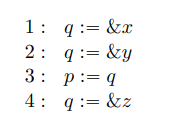
\includegraphics[width=0.3\textwidth]{p145.png}
	\caption{}
	\label{fig:p145}
\end{figure}

After processing the first three statements, Steensgaard’s algorithm will have unified variables
x and y, with p and q both pointing to the unified node. In contrast, Andersen’s algorithm will
have both p and q pointing to both x and y. When the fourth statement is processed, Steensgaard’s
algorithm does only a constant amount of work, merging z in with the already-merged xy node.
On the other hand, Andersen’s algorithm must not just create a points-to relation from q to z, but
must also propagate that relationship to p. It is this additional propagation step that results in the
significant performance difference between these algorithms.


Analyzing Steensgaard’s pointer analysis for efficiency, we observe that each of n statements
in the program is processed once. The processing is linear, except for find operations on the unionfind data structure (which may take amortized time $O(\alpha(n))$ each) and the join operations. We
note that in the join algorithm, the short-circuit test will fail at most $O(n)$ times—at most once for
each variable in the program. Each time the short-circuit fails, two abstract locations are unified,
at cost $O(\alpha(n))$. The unification assures the short-circuit will not fail again for one of these two
variables. Because we have at most $O(n)$ operations and the amortized cost of each operation
is at most $O(\alpha(n))$, the overall running time of the algorithm is near linear: $O(n * \alpha(n))$. Space
consumption is linear, as no space is used beyond that used to represent abstract locations for all
the variables in the program text.

Based on this asymptotic efficiency, Steensgaard’s algorithm was run on a 1 million line program (Microsoft Word) in 1996; this was an order of magnitude greater scalability than other
pointer analyses known at the time.
Steensgaard’s pointer analysis is field-insensitive; making it field-sensitive would mean that it
is no longer linear.


\subsection{Adding Context Sensitivity to Andersen’s Algorithm}

We can define a version of Andersen’s points-to algorithm that is context-sensitive. In the following approach, we analyze each function separately for each calling point. The analysis keeps track
of the current context, the calling point n of the current procedure. In the constraints, we track
separate values for each variable $x_n$ according to the calling context n of the procedure defining it,
and we track separate values for each memory location $l_n^k$ according to the calling context n active
when that location was allocated at new instruction k. The rules are as follows:


\begin{figure}[H]
	\centering
	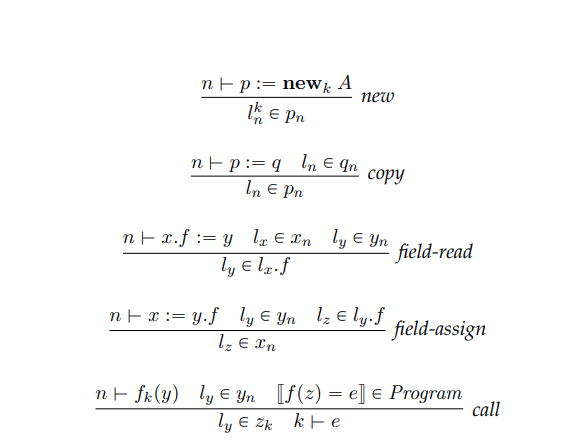
\includegraphics[width=0.3\textwidth]{p146.png}
	\caption{}
	\label{fig:p146}
\end{figure}


To illustrate this analysis, imagine we have the following code:

\begin{figure}[H]
	\centering
	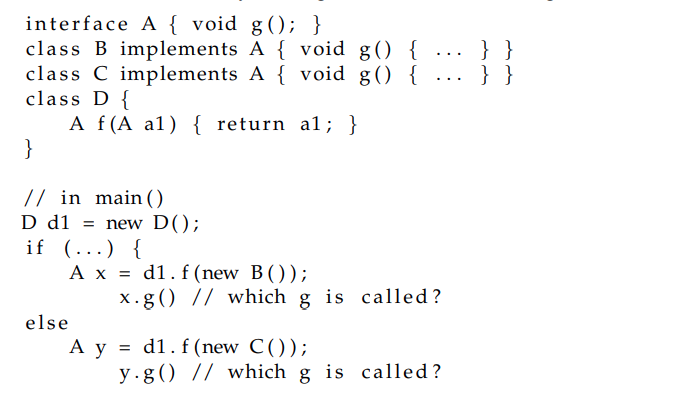
\includegraphics[width=0.3\textwidth]{p147.png}
	\caption{}
	\label{fig:p147}
\end{figure}

The analysis produces the following aliasing graph:


\begin{figure}[H]
	\centering
	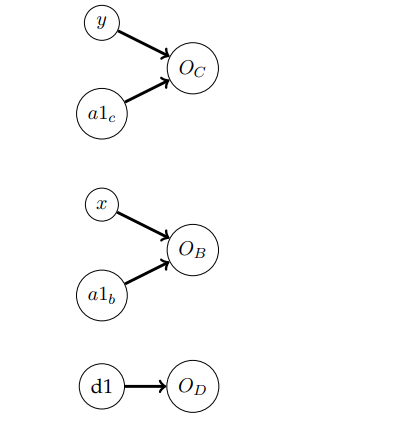
\includegraphics[width=0.3\textwidth]{p148.png}
	\caption{}
	\label{fig:p148}
\end{figure}


In this example, tracking two separate versions of the variable a1 is sufficient to distinguish
the objects of type B and C as they are passed through method f, meaning that the analysis can
accurately track which version of g is called in each program location.

Call-string context sensitivity has its limits, however. Consider the following example,
adapted from notes by Ryder:

\begin{figure}[H]
	\centering
	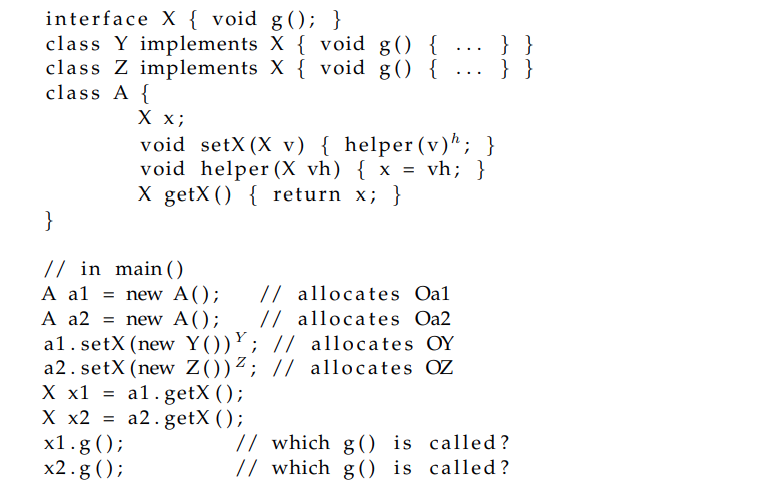
\includegraphics[width=0.3\textwidth]{p149.png}
	\caption{}
	\label{fig:p149}
\end{figure}


If we analyze this example with a 1-CFA style call-string sensitive pointer analysis, we get the
following analysis results:


\begin{figure}[H]
	\centering
	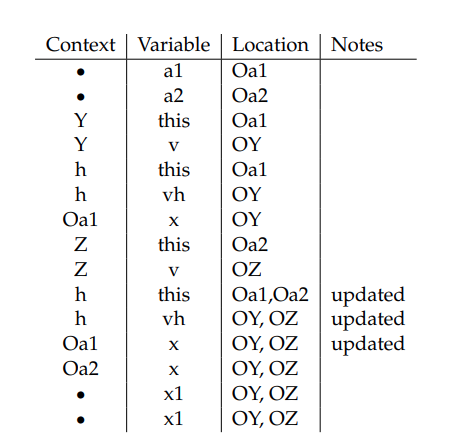
\includegraphics[width=0.3\textwidth]{p150.png}
	\caption{}
	\label{fig:p150}
\end{figure}


Essentially, because of the helper method, one function call’s worth of context sensitivity is
insufficient to distinguish the calls to setX and helper for the objects Oa1 and Oa2. We could fix
this by increasing context sensitivity, e.g. by going to a 2-CFA analysis that tracks call strings of
length two. This has a very high cost in practice, however; 2-CFA does not scale well to large
object-oriented programs.

A better solution comes from the insight that in the above example, call-strings are really tracking the wrong kind of context. What we need to do is distinguish between Oa1 and Oa2. In other
words, the call chain does not matter so much; we want to be sensitive to the receiver object.

An alternative approach based on this idea is called object-sensitive analysis. It uses for the
context not the call site, but rather the receiver object. In this case, we index everything not by a
calling point n but instead by a receiver object l. The rules are as follows:


\begin{figure}[H]
	\centering
	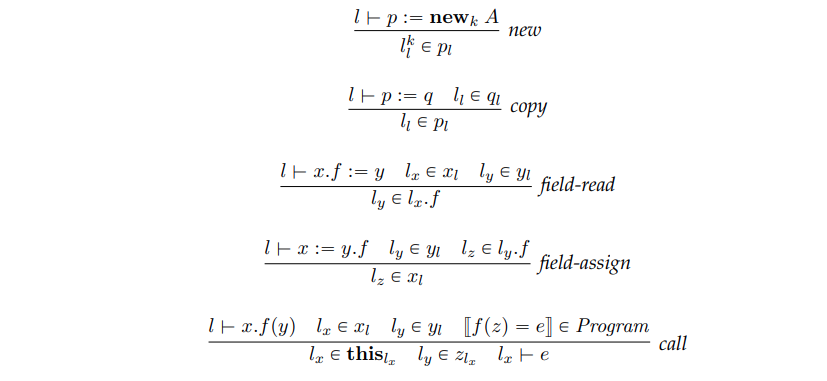
\includegraphics[width=0.5\textwidth]{p151.png}
	\caption{}
	\label{fig:p151}
\end{figure}


Now if we reanalyze the example above, we get:


\begin{figure}[H]
	\centering
	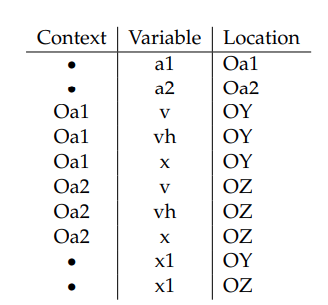
\includegraphics[width=0.3\textwidth]{p152.png}
	\caption{}
	\label{fig:p152}
\end{figure}

In practice, object-sensitive analysis appears to be the best approach to context sensitivity in
the pointer or call-graph construction analysis of object-oriented programs. Intuitively, it seems
that organizing a program around objects makes the objects themselves the most interesting thing
to analyze.

The state of the art implementation technique for points-to analysis of object-oriented programs was presented by Bravenboer and Smaragdakis in OOPSLA 2009. Their approach generates declarative Datalog code to represent the input program, and a datalog evaluation engine
solves what are essentially declarative constraints to get the analysis result.

In an more recent POPL 2011 paper analyzing object-sensitivity, Smaragdakis, Bravenboer,
and Lhotak demonstrate that it is more effective than call-string sensitivity. They also propose a ´
technique known as type-sensitive analysis which tracks only the type of the receiver (and, for
depths $\geq$ 2, the type of the object that created the reciever, etc.), and show that type-sensitive
analysis is nearly as precise as object-sensitive analysis and much more scalable.
